\documentclass [a4paper, 12pt]{article}


\usepackage{amssymb}
\usepackage{epsfig}
\usepackage{times}
\usepackage{float}
\usepackage[usenames,dvipsnames]{color}
\usepackage{ragged2e}
\usepackage[round,sort&compress]{natbib} 
\usepackage{multicol}
\usepackage{pgfgantt}
\usepackage{hyperref}
\usepackage{graphicx}
\usepackage{subcaption}
\usepackage[ddmmyyyy]{datetime}
\setlength\columnsep{6cm}
\usepackage[top=2cm, bottom=2cm, left=2cm, right=2cm]{geometry}
\setlength{\headsep}{1cm}
\setlength{\footskip}{1cm}
\setlength{\parindent}{1cm}

\setlength{\bibsep}{-2pt}

\def\LCDM{\mbox{$\Lambda$CDM}}
\def\kms{\rm km\ s^{-1}}
\def\hkpc{\mbox{$\rm h^{-1}$kpc}}
\def\hMpc{\mbox{$\rm h^{-1}$Mpc}}
\def\hGpc{\mbox{$\rm h^{-1}$Gpc}}
\def\hMsun{\mbox{$\rm h^{-1}$M$_\odot$}}
\def\lesssim{_ <\atop{^\sim}}
\def\gtsim{_ >\atop{^\sim}}

\hypersetup{hidelinks=true}
\newcommand{\aladin}{{\textsc{A}{ladin}}}
\newcommand{\topcat}{{\textsc{Topcat}}}
\newcommand{\cassis}{{\textsc{Cassis}}}
\newcommand{\simbad}{{\textsc{SIMBAD}}}
\newcommand{\vizier}{{\textsc{v}izie\textsc{r}}}
\renewcommand{\dateseparator}{.}


\begin{document}


\begin{center}
\includegraphics[width=0.3\textwidth]{../images/logo_euro.png} 
\hspace{5cm}
\includegraphics[width=0.4 
\textwidth]{../images/logo_asterics.png}\\
\vspace{1.5cm}
\begin{Huge} \textbf{ASTERICS - H2020 - 653477} \end{Huge} \end{center}


\vspace{1cm}
\Huge
\begin{center}
\bf An introduction to the \\ CDS services and tools\\
\end{center}


\vspace{1cm}
\large
\begin{center}
Ada Nebot Gomez-Moran, Mark Allen and the CDS team\\
\textit{Centre de Donn\'ees astronomiques de Strasbourg, France}
\end{center}
\vspace{0.5cm}
\begin{center}
Jenny G. Sorce\\
\textit{updated with a new template for ASTERICS with the new CDS 
portal, new 
plots}\\
\vspace{0.5cm}
Katharina A. Lutz\\
\textit{updated to \aladin\ v10}
\end{center}
\vspace{0.5cm}
\begin{center}
last update \today
\end{center}


\vspace{3.5cm}
Template by Jenny G. Sorce


\newpage
\normalsize
\vfill
\tableofcontents
\vfill

\newpage

\justify
\section{Introduction}

The CDS harbours three major programs, accessible through the CDS portal:\\
\begin{itemize}
\item 
\includegraphics[width=0.1 \textwidth]{../images/logo_simbad.png} 
\textbf{\simbad}: The astronomical database \simbad\ contains more than 
8 million objects. For each object it provides basic measurements (type, 
coordinates, proper motion, radial velocity, spectral type, distance, 
magnitude), cross-correlations and bibliography.
\item 
\includegraphics[width=0.08  \textwidth]{../images/logo_vizier.png}  
\textbf{\vizier}: The \vizier\ catalogue service provides access to about 
15,000 catalogues, being the most complete library of published astronomical 
data tables available online.
\item 
\includegraphics[width=0.1  \textwidth]{../images/logo_aladin.png} 
\textbf{\aladin}: The interactive sky atlas \aladin\ allows to 
visualize astronomical images and to superimpose entries from different 
catalogues and databases. It allows to visualize \simbad\ and \vizier\ 
information and distributed archives and databases as well as to upload own 
tables or images. There are two versions of \aladin: Aladin desktop and Aladin 
lite which runs in the browser.
\end{itemize}

In addition, the CDS has been offering a cross-match service 
(X-match 
\includegraphics[width=0.03 
\textwidth]{../images/logo_cds_xmatch.png} ) since November 2011. 

\section{Goal of this tutorial}

This tutorial shows how to use the CDS tools to gather information on 
specific astronomical objects. We will:
\begin{itemize}
\item Search for information on NGC4039 in the CDS portal
\item Search for data on NGC4039 in \aladin\
\item Compare the coverage of Sky Surveys and select interacting 
galaxies that have SDSS and GALEX data
\end{itemize}

\section{Search for information on NGC4039 in the CDS Portal}

Open the CDS Portal 
\hyperref[http://cdsportal.u-strasbg.fr/]{\textcolor{blue}{http://cdsportal.u-strasbg.fr/}}
and make a query for `NGC4039'.
The result provides an overview of the information and data available for 
this object in the 3 CDS services: \simbad, \aladin\ and \vizier: 

\begin{figure}[H]
\center
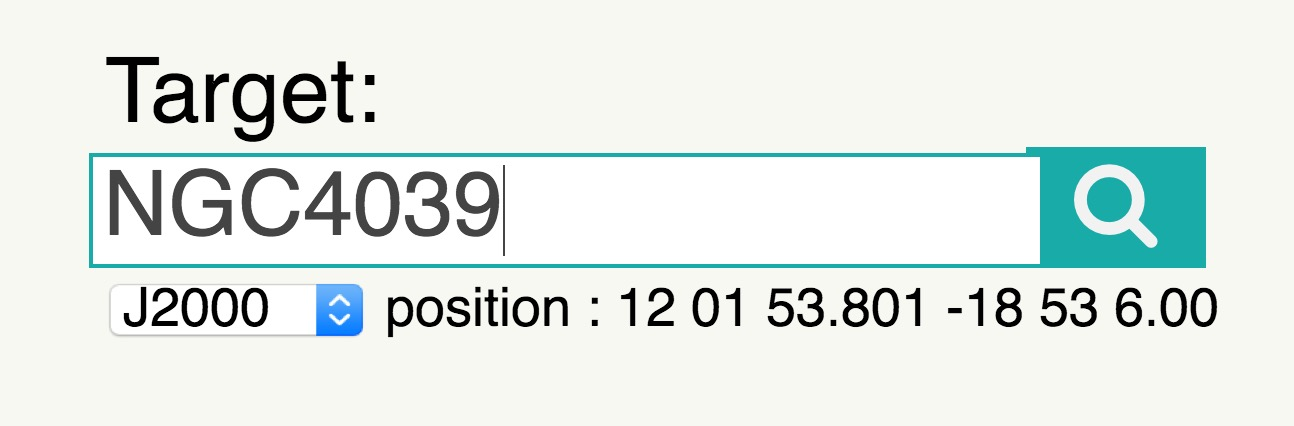
\includegraphics[width=0.5  \textwidth]{../images/cdsportal_search_ngc4039.jpg}
\caption{Query for NGC4039 in the CDS Portal}
\label{fig:cdsportal1}
\end{figure}

\subsection{\simbad\ - Identifiers, Basic Measurements and links to the 
Bibliography}

\begin{figure}[H]
    \center
    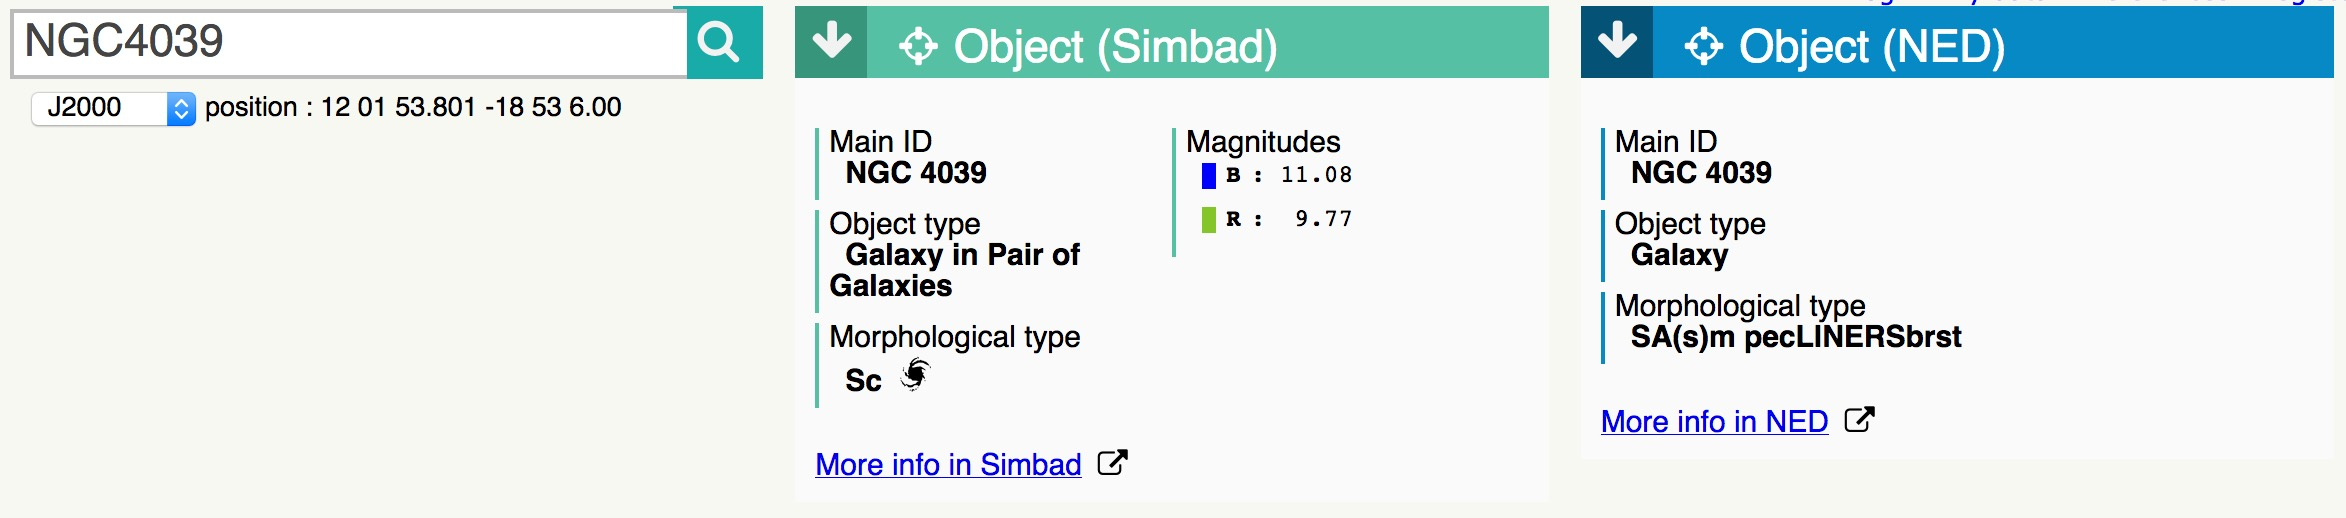
\includegraphics[width=1  
    \textwidth]{../images/cdsportal_object-information_ngc4039.jpg}
    \caption{Result of the query for NGC4039 in the CDS Portal}
    \label{fig:cdsportal2}
\end{figure}

\begin{itemize}
    \item Click on \textbf{More info in Simbad} to see the full \simbad\ 
information on this object in a new tab.
\begin{figure}[H]
    \center
    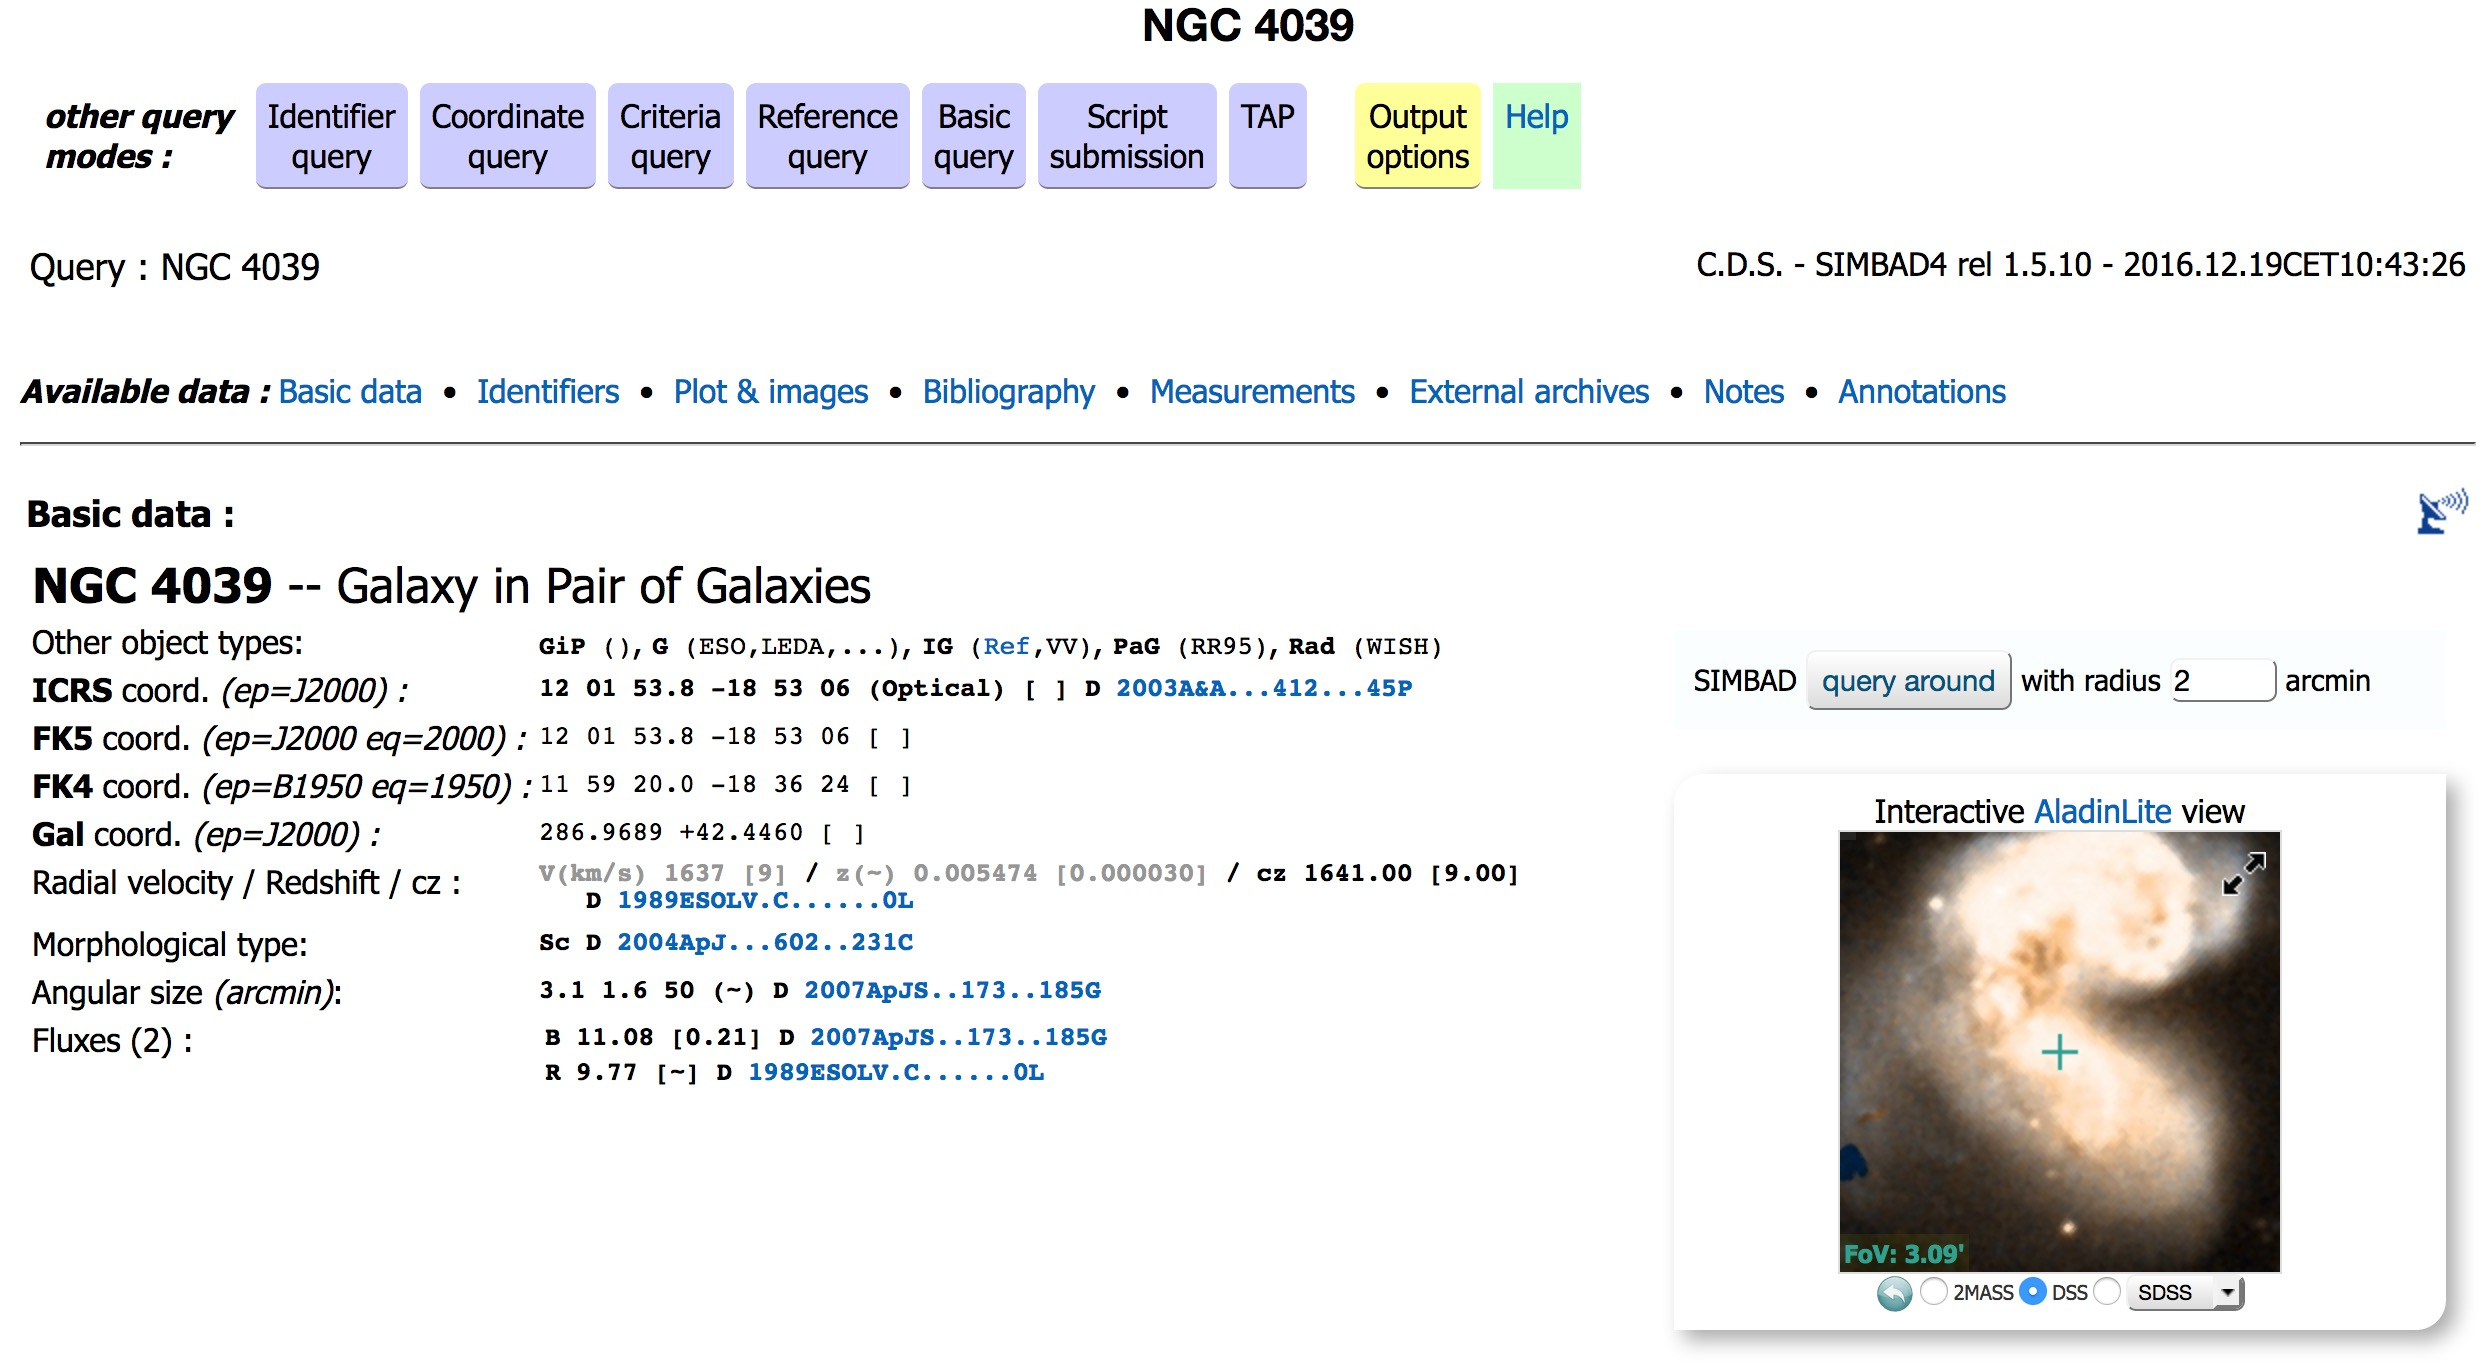
\includegraphics[width=1  
    \textwidth]{../images/simbad_section_basic-data.jpg}
    \caption{Result of the query for NGC4039 in \simbad.}
    \label{fig:simbad}
\end{figure}
    \item Note the list of \textbf{Other object types}. These types are 
drawn for the literature and are stored in \simbad\ using a 
hierarchical classification scheme. The full list of Object Types can 
be found here: 
\hyperref[http://simbad.u-strasbg.fr/simbad/sim-display?data=otypes]
{\textcolor{blue}{http://simbad.u-strasbg.fr/simbad/sim-display?data=otypes}}.
The main Object Type of NGC4039 is \textbf{Galaxy in Pairs of Galaxies 
(GiP)}.
    \item Use the {\bf parents} button 
\includegraphics[width=0.07 
\textwidth]{../images/simbad_button_parents.png} to identify the name 
of the galaxy pair. Sorting by the number of references 

\includegraphics[width=0.04  \textwidth]{../images/simbad_sort_references.jpg} 
can help 
bring out the most important ones. 
    \item Follow the link to the \simbad\ entry of the Antennae galaxy pair 

\includegraphics[width=0.07 
\textwidth]{../images/simbad_antennae-galaxt-pair_link.png}. There 
click on the {\bf children} button 
\includegraphics[width=0.07 
\textwidth]{../images/simbad_button_children.png} to identify the name 
of the two galaxies making up the galaxy pair. Again the number of references 
might help to find them.  
    \item Visit the \simbad\ entry of the interaction partner of NGC\,4039 and 
use the {\bf References} section to find the earliest listed reference in the 
literature to this object.
\begin{figure}[H]
    \center
    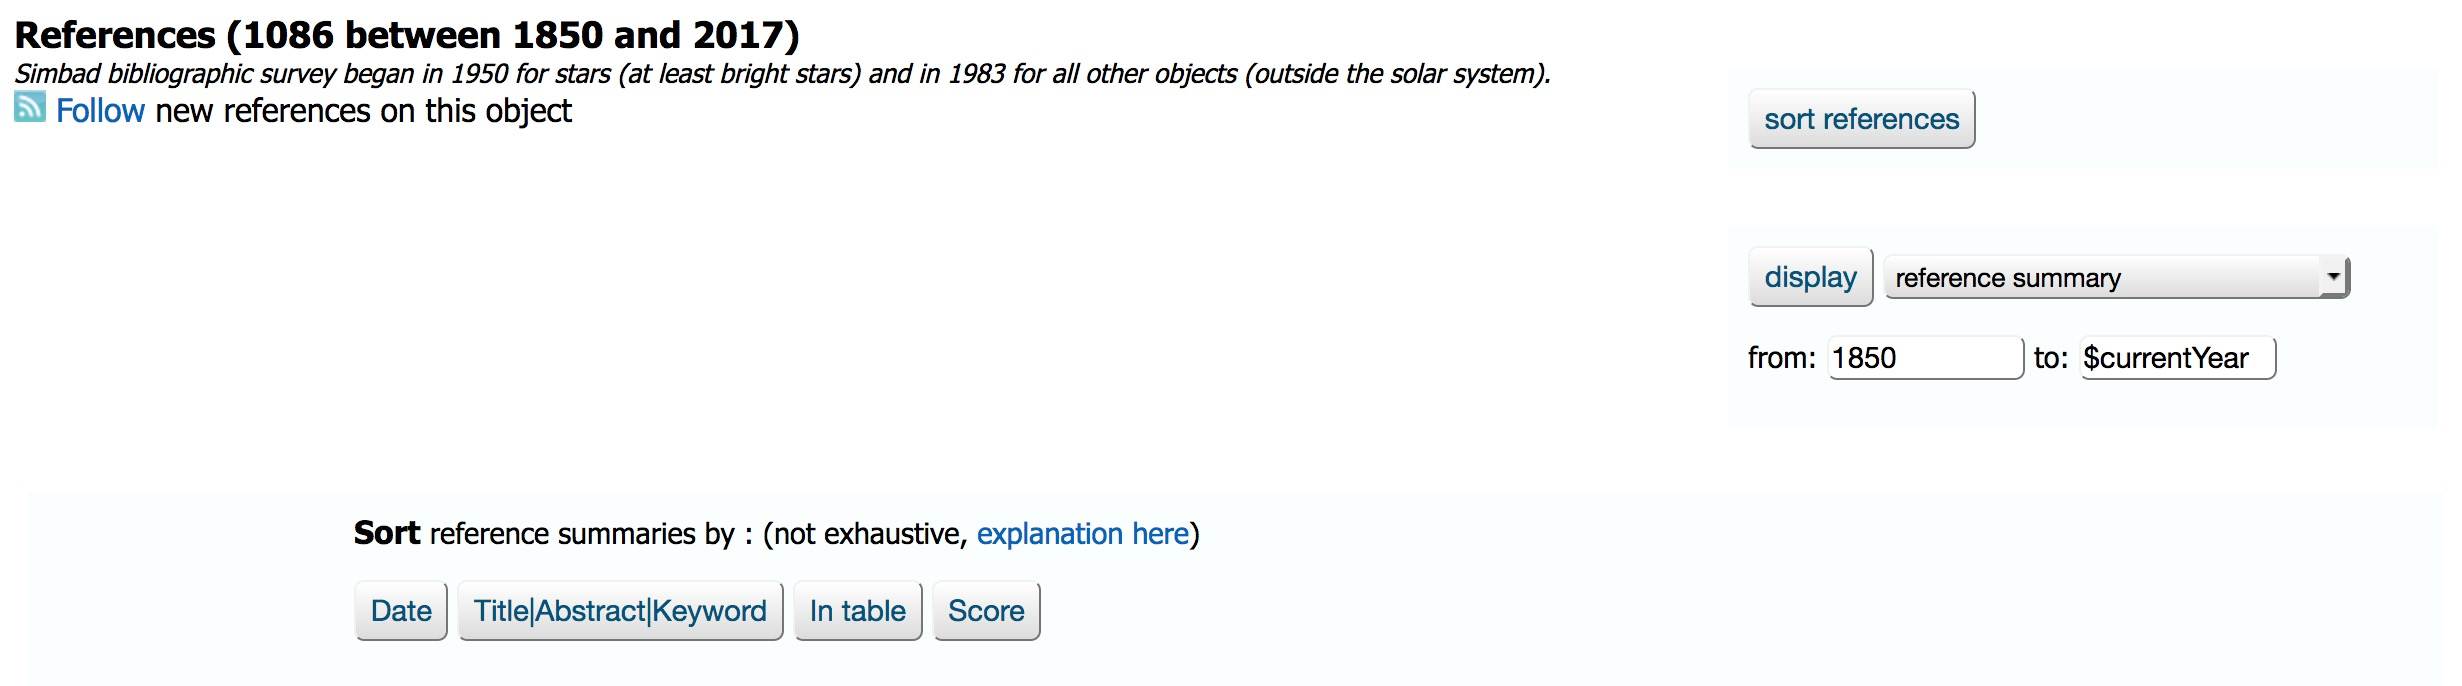
\includegraphics[width=1  
    \textwidth]{../images/simbad_section_references.jpg}
    \caption{References section}
    \label{fig:simbad}
\end{figure}

    \item Return to the CDS portal.
\end{itemize}




\subsection{\aladin\ - Images}


\begin{figure}[H]
\center
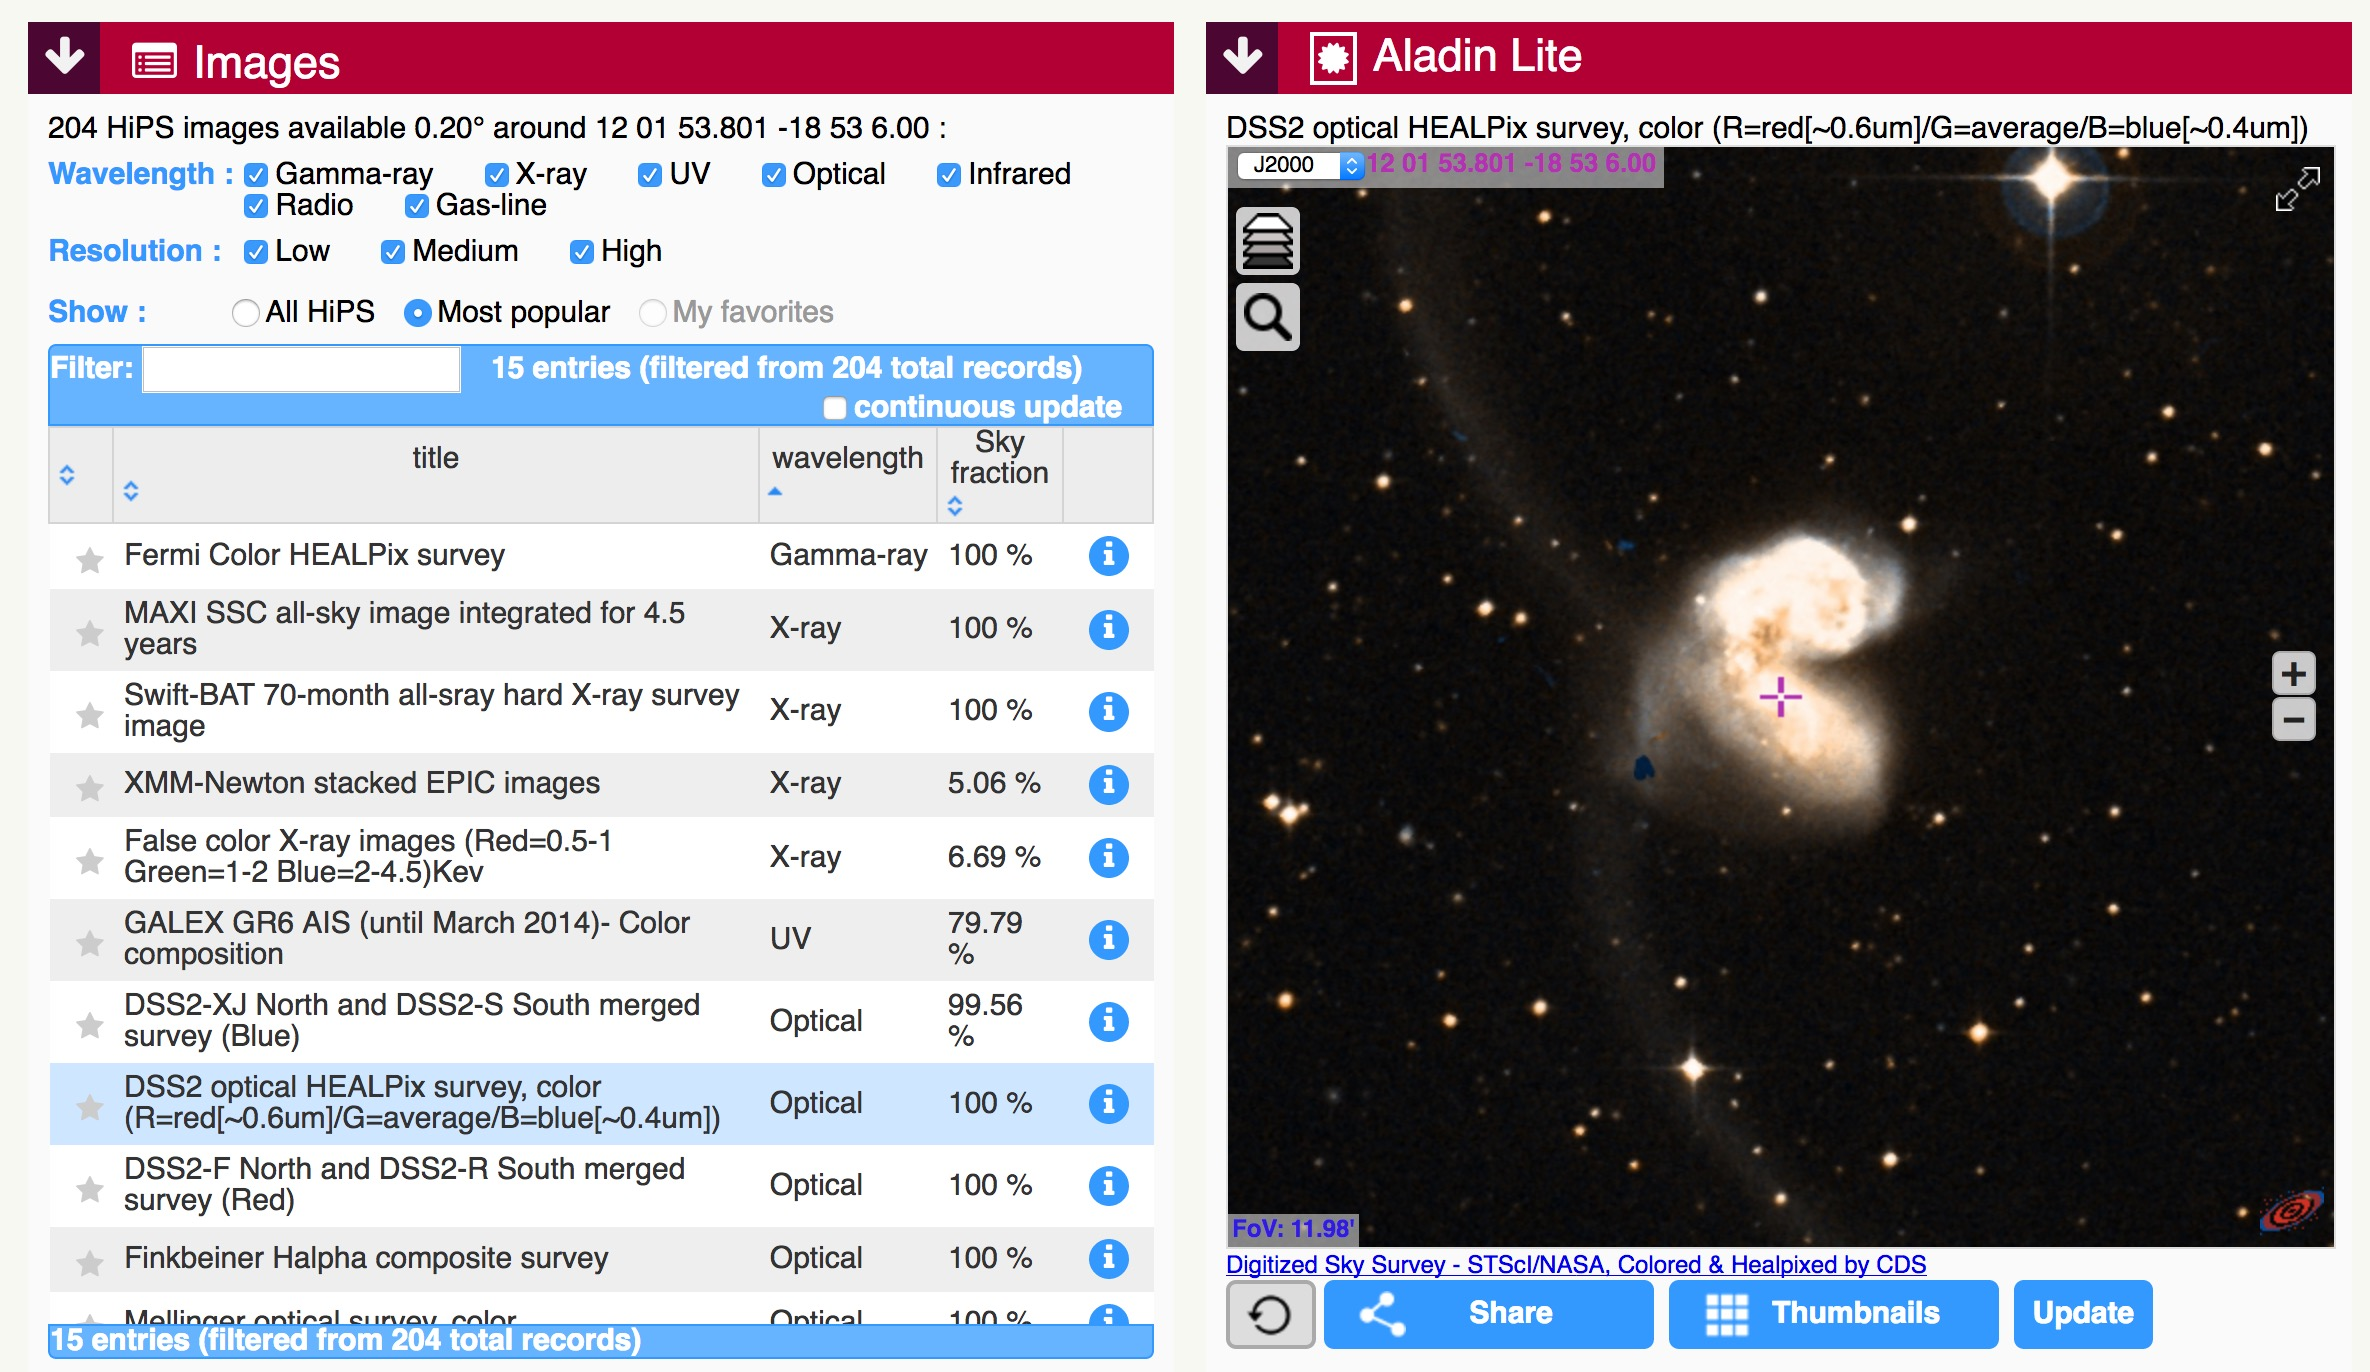
\includegraphics[width=1  
\textwidth]{../images/cdsportal_image-information_ngc4039.jpg}
\caption{Result of the query for NGC4039 in the CDS Portal}
\label{fig:cdsportal3}
\end{figure}

\begin{itemize}
\item A DSS (Digitized Sky Survey) image of NGC4039 is shown.
\item Note that you can zoom in and out by scrolling your mouse when the mouse 
pointer is positioned on top of the images. 
\item Other images can be displayed by selecting them in the left 
column. 
\item Restricted searches on wavelength and resolution are possible by 
ticking/unticking the boxes in that same column.
\end{itemize}


\subsection{\vizier\ - Catalogues}


\begin{figure}[H]
\center
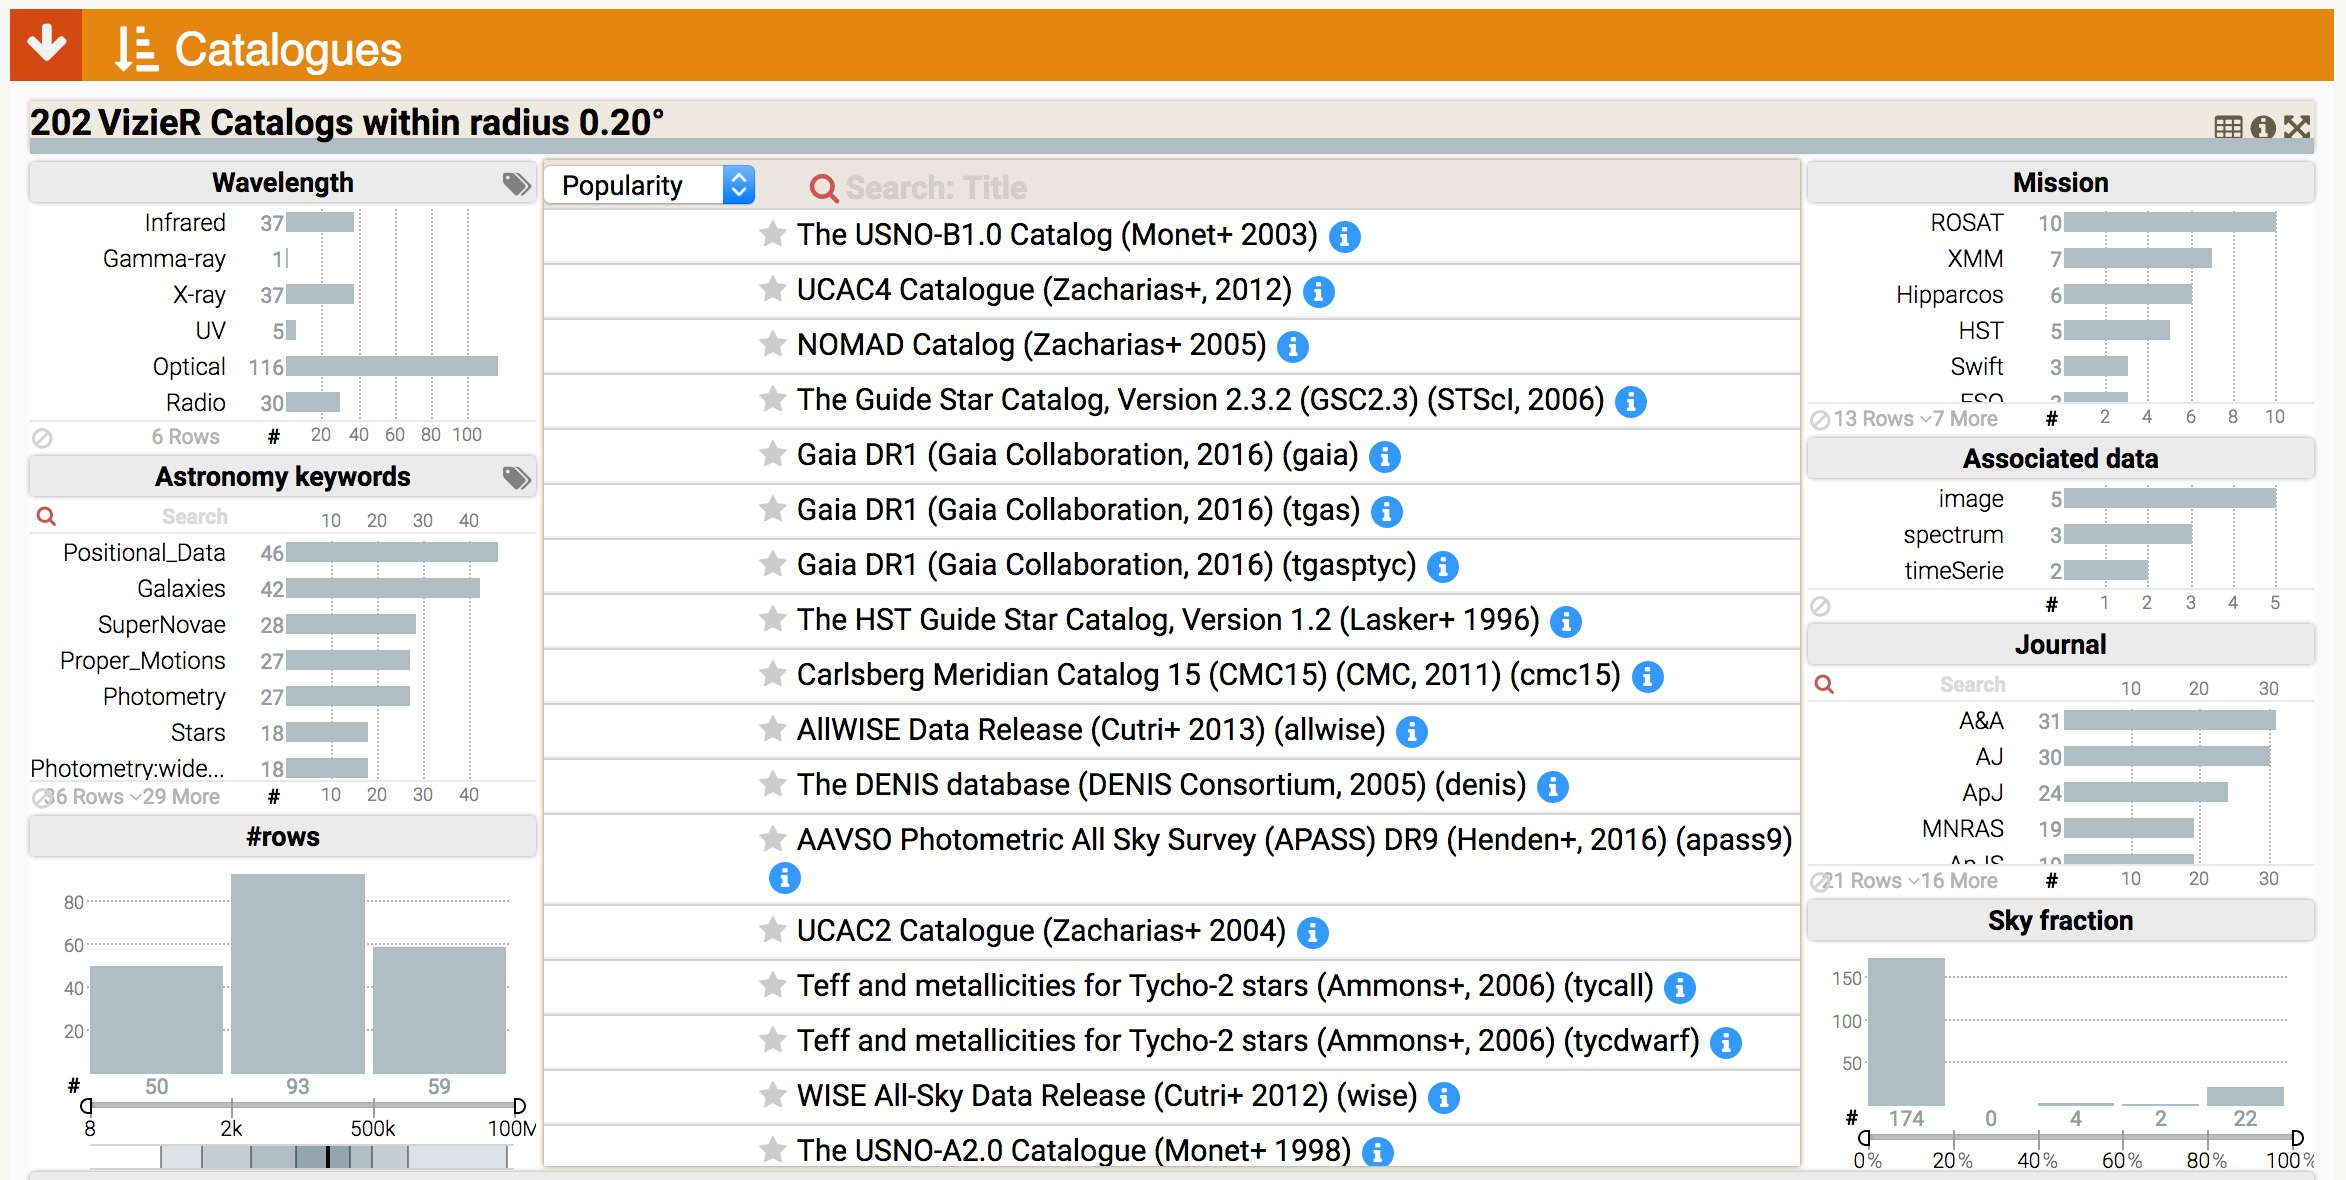
\includegraphics[width=1  
\textwidth]{../images/cdsportal_catalogue-information_ngc4039.jpg}
\caption{Result of the query for NGC4039 in the CDS Portal}
\label{fig:cdsportal4}
\end{figure}

\begin{itemize}
\item The list of catalogues is sorted by \textbf{Popularity} but can 
also be sorted by number of rows (\textbf{\#rows}), \textbf{sky 
fraction} or \textbf{year}. 
\item Note that restrictions and filtering can be applied by clicking 
on the left or right columns according to your wills.
\item After selecting a catalogue, it is possible to visualize it (either 
quickly or in \vizier), to plot it and/or to send it to the \aladin\ 
tool.
\begin{figure}[H]
\center

\includegraphics[width=1  \textwidth]{../images/cdsportal_table_usno.jpg}
\caption{Selection of a \vizier\ Catalogue on the CDS Portal.}
\label{fig:cdsportal5}
\end{figure}
\item Actually the Antennae is listed in the Arp Atlas of Peculiar 
Galaxies, make a search for `Arp' into the \textbf{Search} box.

\begin{figure}[H]
\center
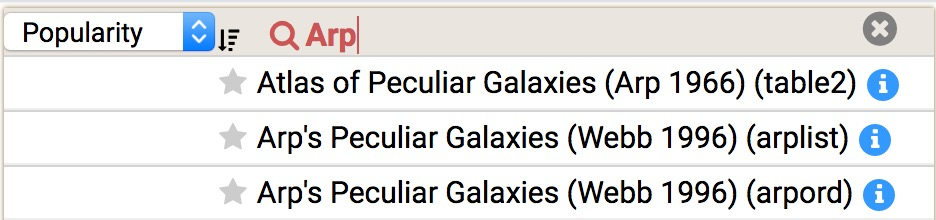
\includegraphics[width=0.6  
\textwidth]{../images/cdsportal_search-table_arp.jpg}
\caption{Looking for `Arp' in the \vizier\ catalogues.}
\label{fig:arp}
\end{figure}
\item Note that there are two tables for Webb 1996. Select the 
\textbf{arplist} 
table by clicking on it and then on 
\includegraphics[width=0.05  
\textwidth]{../images/logo_vizier.png}. This sends to the \vizier\ detailed 
query 
page.
\item Make a first query on this table by clicking on \textbf{submit}. 
Examine the output as html. Go back to the previous page
\item Modify the query preferences to add extra coordinate columns in 
J2000 decimal degrees and to obtain the whole catalogue:
\begin{itemize}
    \item Remove the restriction on searching only around `NGC4039' by clicking 
    on the \textbf{Clear} button below \textbf{Target Name (resolved by 
        Sesame) or Position} at the top of the page. 
    \item In \textbf{Preferences} on the left side of the page, add extra 
    coordinate columns in decimal degrees by ticking \textbf{J2000} and 
    \textbf{decimal} boxes.
    \item Change the maximum (\textbf{max}) number of rows to 
    \textbf{unlimited} and tick \textbf{All columns} to get the whole 
    catalogue
    \begin{figure}[H]
        \center
        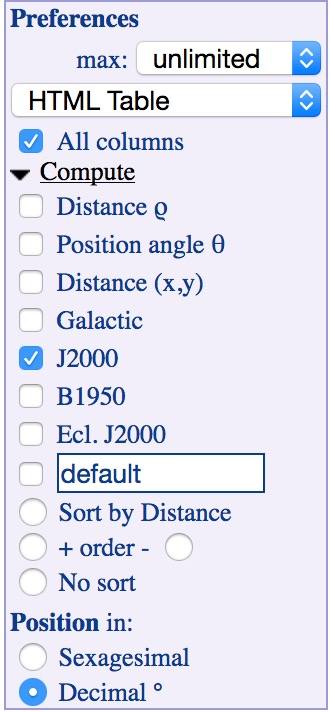
\includegraphics[width=0.2  
        \textwidth]{../images/vizier_preferences.jpg}
        \caption{\textbf{Preferences} panel.}
        \label{fig:pref}
    \end{figure}
    \item Submit again.
\end{itemize}
\end{itemize}
The following steps are optional for the workflow of this tutorial, but they 
might come in handy for other problem sets. 
\begin{itemize}
\item When satisfied, click on \textbf{Save in CDSportal}, then click 
on the \textbf{Save} button. The file is now saved in your personal 
user space on the CDS portal.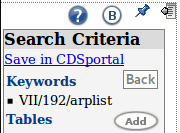
\includegraphics[width=0.1  
\textwidth]{../images/vizier_saveto_CDSportal.png}
\item Click on \textbf{Go to MyData} and download a copy in 
\textbf{VOTable} format on your desktop. This file can be used later 
in the tutorial.
\begin{figure}[H]
\center
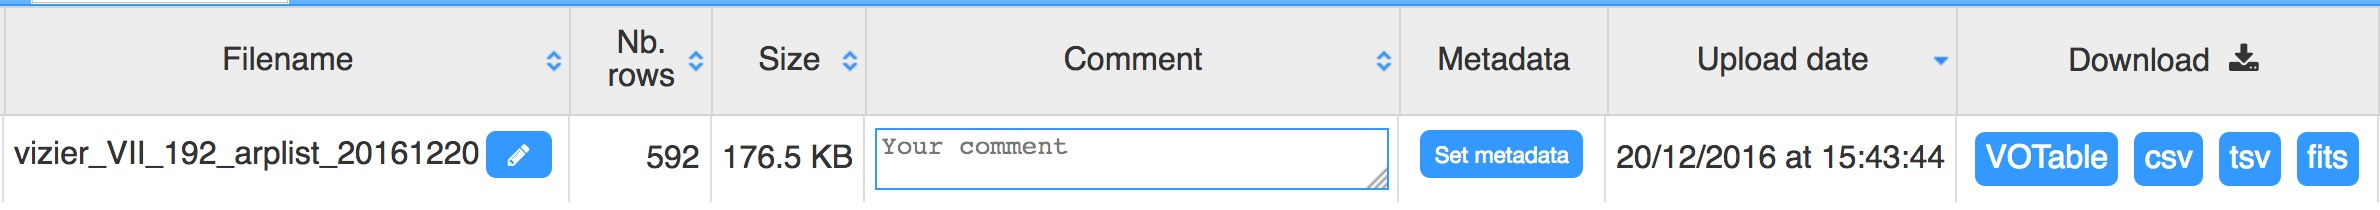
\includegraphics[width=1  \textwidth]{../images/cdsportal_mydata.jpg}
\caption{Personal User Space on the CDS Portal.}
\label{fig:download}
\end{figure}
\end{itemize}

\subsection{How does the data get into the CDS databases?}
As you have seen in the last sections, the CDS databases (\simbad, \vizier, the 
HiPS server for images) host large amounts of a variety of data products. But 
how does the data published in papers find their way into the databases? At the 
CDS, about 12 documentalists work on curating data. This involves collecting 
data from journal papers, receiving data directly from large surveys (such as 
e.\,g. Gaia), assessing and assuring the data quality and cross-matching 
sources described by newly published papers/data with sources already available 
in the databases. You can make this a smooth process by making sure that all 
sources in your papers appear with correct coordinates and names already known 
by \simbad. 

\section{Search for data on NGC4039 in \aladin}

Open \aladin\ with at least 1GB memory allocated to the save virtual 
machine. To do so use the following command line: \texttt{java -Xmx1024m -jar 
Aladin.jar}

Aladin offers two ways to retrieve data: through the \textsc{Data Tree} on the 
left hand side of the \aladin\ window and through the 
\textsc{Server Selector} window, which can be opened via \textbf{File 
$\rightarrow$ Open server selector...} or with \textbf{CTRL + l}. 

Data sets in the \textsc{Data Tree} are colour coded in green or orange 
depending on whether or not they are available in the region currently visible 
in the main viewing window. 

\begin{figure}[H]
    \centering
    \begin{subfigure}[H]{0.4\textwidth}
        \center
        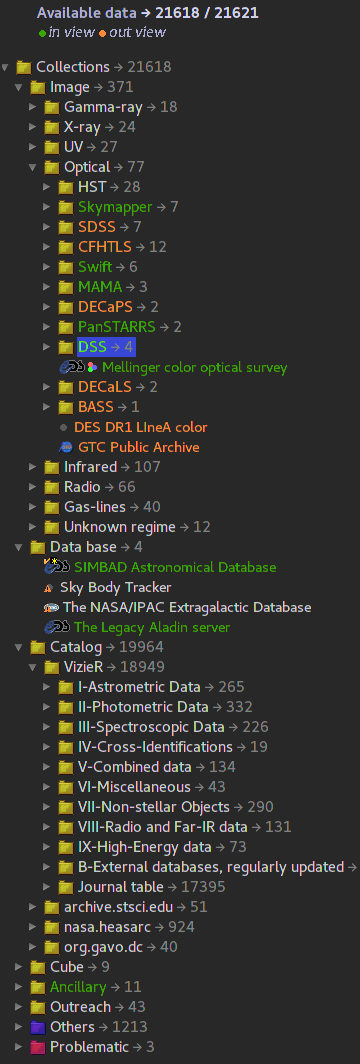
\includegraphics
            [width=0.4\textwidth]
            {../images/aladin_data_discovery_tree_open.png}
        \caption{The \textsc{Data Tree}: green entries are available for the 
        sky region currently visible in the main viewing window (not shown).}
        \label{fig:data_disc_tree}
    \end{subfigure}
    \centering
    \begin{subfigure}[H]{0.4\textwidth}
        \center
        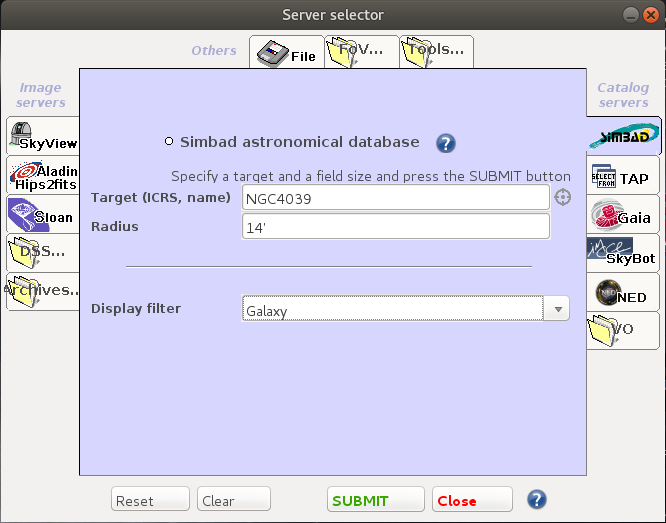
\includegraphics[width=1 
        \textwidth]{../images/aladin_server_selector.png}
        \caption{The \textsc{Server Selector} window: here \simbad\ has been 
        queried for galaxies within 14\,arcmin around NGC\,4093.}
        \label{fig:server_selector}
    \end{subfigure}
    \caption{The two entry points to retrieving data in Aladin: The 
    \textsc{Data Tree} (left) and the \textsc{Server Selector} (right).}
\end{figure}

\begin{itemize}
    \item Start by typing "NGC4039" in the \textbf{Command} line 

\includegraphics[width=0.2\textwidth]{../images/aladin_command_ngc4039.png} 
and press \textbf{Enter}. In the main viewing window the coloured DSS image of 
the Antennae galaxies appears. As for the \aladin\ lite window in the CDS 
portal you can zoom in and out by scrolling your mouse. 

    \item Make a contour map of the image using the \textbf{cont} button 

\includegraphics[width=0.03  \textwidth]{../images/aladin_button_contours.png} 
next to main viewing window. Increase the number of contours to better 
represent the image. 
    
    \item Overlay a \simbad\ plane showing only the galaxies by selecting 
the 
\includegraphics[width=0.055  \textwidth]{../images/logo_simbad.png} tab  
in 
the 
\textsc{Server selector} and choosing \textbf{Galaxy} as the \textbf{Display 
filter} (see Figure~\ref{fig:server_selector}).

    \item Change the colour of the \simbad\ plane using the button 
\textbf{Properties} 

\includegraphics[width=0.03\textwidth]{../images/aladin_button_properties.png}. 
 

    \item Using the \textbf{Select} tool 
\includegraphics[width=0.03  
\textwidth]{../images/aladin_button_select.png}, select some of the \simbad\ 
points either by clicking on one point or by holding the left mouse button and 
drawing a rectangle. The sources within the rectangle are then selected and 
displayed as a table below the image. This window can be detached with the icon 

\includegraphics[width=0.035  
\textwidth]{../images/aladin_button_detach-table.png} in the bottom right 
corner of the table window. Note that the data point 
belonging to a row in the table blinks in the main viewing window when 
hoovering over the table row with the mouse.

    \item In the \textsc{Data Tree}, go to \textbf{Images $\rightarrow$ 
Infrared $\rightarrow$ 2MASS} and load the 2MASS colour image. To so click on 
the 2MASS colour image entry and the loading window appears (see 
Figure~\ref{fig:aladin_load_2mass}). In the loading window, check that the box 
for progressive loading is ticked 
\includegraphics[width=0.07   
\textwidth]{../images/aladin_load_progessive.png} and load the image by 
clicking \textbf{Load}  
\includegraphics[width=0.07   
\textwidth]{../images/aladin_load_load.png}.

\begin{figure}[H]
    \center
    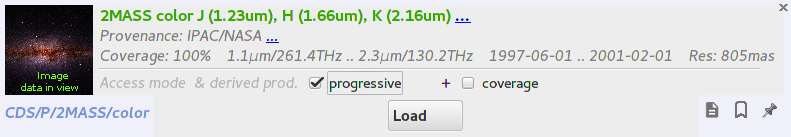
\includegraphics[width=1  
    \textwidth]{../images/aladin_load_2mass-rgb-image.png}
    \caption{Loading the 2MASS colour image from the \textsc{Data Tree}. }
    \label{fig:aladin_load_2mass}
\end{figure}

    \item Once the 2MASS image is loaded in appears in the stack, which is 
    located to the right of the main viewing window. The stack informs you of 
    all planes that are currently loaded into \aladin. These layers are shown 
    in the main viewing window as if you were looking from top to bottom 
    through the stack. Now being most recently loaded, the 2MASS plane is shown 
    as the "background" image in the main viewing window. If you now want to go 
    back to the DSS colour image being the "background" image, tick the little 
    grey box next to the DSS image entry in the stack. If you now use the 
    opacity slider 
\includegraphics[width=0.035  
    \textwidth]{../images/aladin_button_opacity.png} next to the 2MASS plane in 
    the image stack, you can change opacity of the 2MASS plane and thus compare 
    it easily to the DSS image. If you wanted to overlay the DSS image on the 
    2MASS image, you would have to change their order in the stack by drag-and 
    drop. 

    \item Now add more colour images form the \textsc{Data Tree}, for example 
the allWISE (infrared) and the XMM Newton (X-rays) colour images. Compare the 
images in a number of different ways:
    \begin{itemize}
        \item Multiview: \textbf{View $\rightarrow$ Create one view per image}, 
        or via the \textbf{multiview} icon at the bottom left of the \aladin\ 
        image window 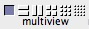
\includegraphics[width=0.1 
        \textwidth]{../images/aladin_button_multiview.jpg}. After selecting 
        e.\,g. the four by four grid drag and drop the images into the panels, 
        where you want to see them. 
        \item Align and scale all images by using the \textbf{match} icon below 
        the image window 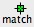
\includegraphics[width=0.04  
        \textwidth]{../images/aladin_button_match-views.jpg}. 
        \item Transparency overlays: return to single view mode. Change the 
        transparency of planes in the stack with the opacity sliders         
        
\includegraphics[width=0.04  
        \textwidth]{../images/aladin_button_opacity.png} as before. Remember  
        that you can move the location of the planes in the stack and thus 
        change the order in which the image are shown.
    \end{itemize}
    
    \item All the colour images we have loaded so far are pre-computed.
\aladin\ also allows you to compute your own RGB colour images:
     \begin{itemize}
         \item For this task, we need fits images rather the HiPS tiles we have 
         worked with so far. Those fits images may come from your own data or 
         from the Virtual Observatory. We will now search and load images at 
         the location of the Antennae galaxies from the VO. 
         \item First, we look for a far-ultraviolet image from 
         \textit{GALEX}, enter "GALEX Atlas of nearby galaxies" in the 
         \textbf{Select} line below the 
         \textsc{Data Tree} 
\includegraphics[width=0.17  
         \textwidth]{../images/aladin_select_GALEX.png}. In the \textsc{Data 
         Tree} you will find the entry "GALEX Atlas of nearby galaxies" under 
         \textbf{Others} $\rightarrow$ \textbf{SIA (image)} $\rightarrow$ 
         \textbf{mast.stsci}. Load this entry \textbf{in view} 
         
\includegraphics[width=0.07 
         \textwidth]{../images/aladin_load_inview.png}. A table appears in the 
         stack. 
         \item The newly loaded table contains a row for every image available 
         from this image service in the vicinity of NGC\,4039. Find the entry 
         for the file "h\_ngc4038-fd-int.fits.gz" and click on the URL in the 
         first column. This will load the corresponding fits image into your 
         stack. 
%         \item Empty the \textbf{Select} line and repeat the steps from above 
%         to load a $R$-band image from the Digitised Sky Survey: go to 
%         \textbf{Others} $\rightarrow$ \textbf{SIA (image)} $\rightarrow$ 
%         \textbf{eso.org} and load the table of observations of the 
%         \textbf{Digitized Sky Survey}. In the newly loaded table select the 
%         row with "SurveyName" "DSS2-red" and load the corresponding image 
%         from 
%         the URL in the first column. 
         \item Next, we are after an infrared image: search for "2MASS large 
         galaxy atlas" in the \textbf{Select} line, load the table from 
         \textbf{Others} $\rightarrow$ \textbf{SIA (image)} $\rightarrow$ 
         \textbf{irsa.ipac} and select any one of the three entries in the 
         table to load into the stack.
         \item Finally let's add an X-ray image to the collection: search for 
         "XMM-Newton Pointed" in the \textbf{Select} line, load the table from 
         \textbf{Others} $\rightarrow$ \textbf{SIA (image)} $\rightarrow$ 
         \textbf{esavo} and select the observation with the longest "Duration".
         \item To create the RGB image, open the \textbf{RGB image generator} 
         with 
\includegraphics[width=0.04  
         \textwidth]{../images/aladin_button_rgb.png} (see 
         Figure~\ref{fig:aladin_rgb_generator}). Enter the images you want to 
         use for each colour component and click
     \end{itemize}

\begin{figure}[H]
    \centering
    \begin{subfigure}[H]{0.4\textwidth}
        \center
        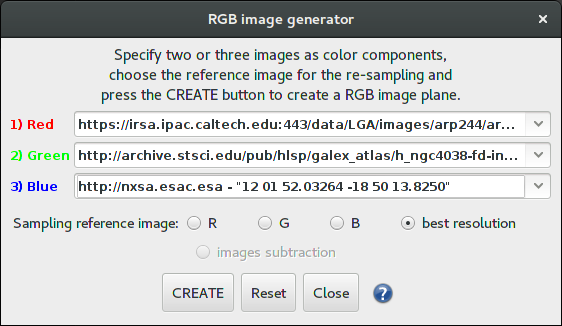
\includegraphics
        [width=\textwidth]
        {../images/aladin_rgb_window.png}
        \caption{The RGB image generator window. }
           \label{fig:aladin_rgb_generator}
       \end{subfigure}
       \centering
       \begin{subfigure}[H]{0.4\textwidth}
           \center
           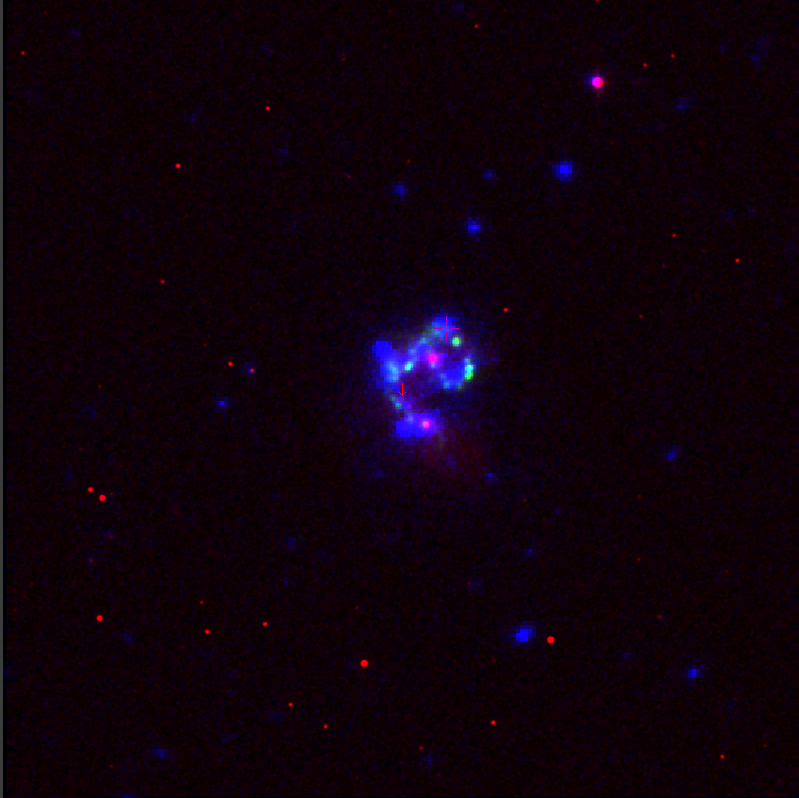
\includegraphics[width=1 
           \textwidth]{../images/aladin_results_rgb_image.png}
           \caption{The resulting RGB image for the Antennae galaxies. }
           \label{fig:rgb_image}
       \end{subfigure}
       \caption{Creating RGB images in \aladin.}
   \end{figure}     

    \item Search for more data from the VO on NGC4039:
    \begin{itemize}
        \item To restrict the collections that the \textsc{Data Tree} is 
        showing, use the \textbf{Select} line below the 
        \textsc{Data Tree} 
\includegraphics[width=0.1  
        \textwidth]{../images/aladin_select_transient.png}. For example when 
        searching for transients within 
        the Antennae galaxies you might restrict the search to "transient" and 
        find that the Palomar Transient Factory photometric catalogue has data 
        for transient events in the area. Load the catalogue and find the data 
        points in the main viewing window. 
        \item More elaborate filters can be created using the \textbf{Data 
        Discovery Tree Filter} window, accessed through 
        
\includegraphics[width=0.04  
        \textwidth]{../images/aladin_button_filtertree.png} next to the 
        \textbf{Select} line.
        \item As before, entries in the \textsc{Data Tree}, which are coloured 
        in green, have data available in the region currently visible in the 
        main viewing window.  
    \end{itemize}
    \item Now delete all the planes in your stack before continuing. This is 
    not mandatory but it will free some useful memory space and allow you to 
    proceed more easily with the next steps.
\end{itemize}    
\begin{figure}[H]
\center
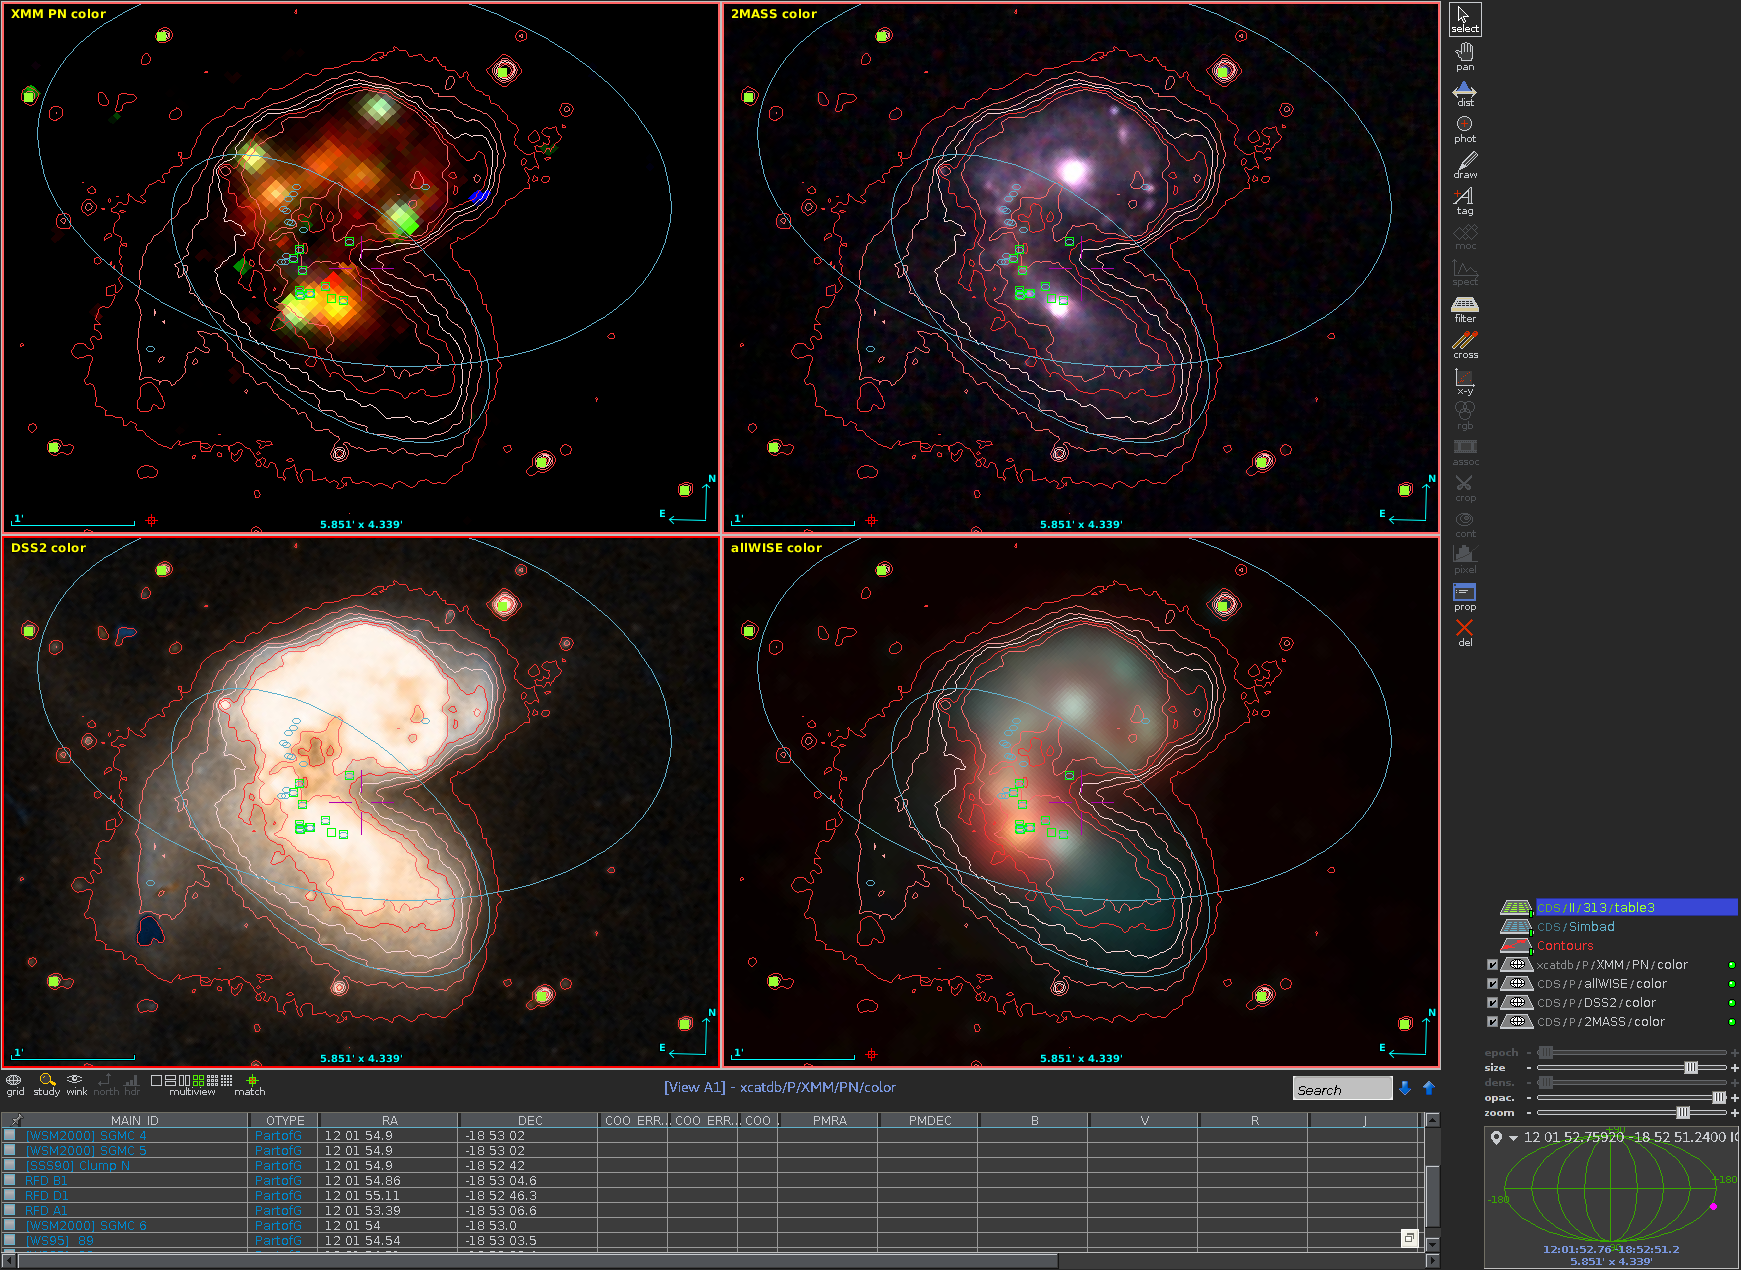
\includegraphics[width=0.7  
\textwidth]{../images/aladin_results_cdstutorial-sec4.png}
\caption{Results of all the above mentioned steps.}
\label{fig:aladinNGC4039}
\end{figure}


\section{Compare the coverage of Sky Surveys and select interacting 
galaxies that have SDSS and GALEX data}

Many large sky surveys in \aladin\ are stored in the \textbf{HiPS} format
(Hierarchical Progressive Survey, see 
\hyperref[http://aladin.u-strasbg.fr/hips/]{\textcolor{blue}
	{http://aladin.u-strasbg.fr/hips/}}),
which allows for easy access, browsing and visualisation of image and catalogue 
data. To describe (non-trivially shaped) regions on the sky \textbf{MOC} 
(Multi-Order Coverage) maps are used. In the following, we will make use of the 
advantages of these two data structures to easily asses which galaxies in the 
Arp catalogue of peculiar galaxies have been observed by SDSS and GALEX. If you 
would like to have an overview of currently available HiPS, have a look at 
\hyperref[https://aladin.u-strasbg.fr/hips/list]{\textcolor{blue}
	{https://aladin.u-strasbg.fr/hips/list}}. You can load any of them in 
\aladin\ by entering their base URL in the \textbf{Command} line.  

\begin{itemize}
    \item Select the \textbf{SDSS 9 colored} (\textbf{Image $\rightarrow$ 
Optical $\rightarrow$ SDSS}) and \textbf{GALEX All Sky Imaging Survey 
colored} (\textbf{Image $\rightarrow$ UV $\rightarrow$ GALEX}) surveys in the 
\textsc{Data Tree} and load both the imaging data (tick progressive 

\includegraphics[width=0.1\textwidth]{../images/aladin_load_progessive.png}) 
and the MOC of the survey (tick coverage

\includegraphics[width=0.1\textwidth]{../images/aladin_load_coverage.png}). For 
the moment make the two MOC planes invisible by clicking on their opacity slider

\includegraphics[width=0.04\textwidth]{../images/aladin_button_opacity.png}.
\begin{figure}[H]
\center
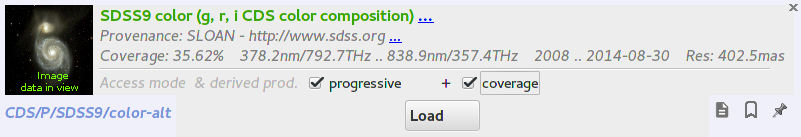
\includegraphics[width=0.7  
\textwidth]{../images/aladin_load_sdss-image-moc.png}
\caption{Selecting the SDSS 9 coloured survey and MOC}
\label{fig:aladinselect}
\end{figure}

    \item Turn on the coordinate \textbf{grid} 

\includegraphics[width=0.035\textwidth]{../images/aladin_button_grid.jpg}, zoom 
out and use 
the \textbf{pan} tool 
\includegraphics[width=0.035\textwidth]{../images/aladin_button_pan.png} to 
explore the whole sky.

    \item Now turn the MOC planes back on (click again on the opacity slider).
Zoom onto the edges of the surveys and note the way the MOC represents the 
coverage of the surveys.

    \item Calculate the intersection of the coverage maps of the SDSS and 
GALEX surveys using in the menu the item \textbf{Coverage $\rightarrow$ 
Logical operations} or the MOC button 
\includegraphics[width=0.035\textwidth]{../images/aladin_button_moc.png} on the 
right of the main viewing window. 

\begin{figure}[H]
\center
\includegraphics[width=0.4 \textwidth]{../images/aladin_moc_intersection.jpg}
\caption{Building the intersection of the coverage maps}
\label{fig:intersec}
\end{figure}

    \item Load the full Webb 1996 Arp catalogue that you saved earlier. You 
can do this in one of the following three ways:
    \begin{itemize}
        \item \textbf{File $\rightarrow$ Load local file... }.
        \item Drag and drop on the stack.
        \item Broadcast the catalogue from the \vizier\ page that shows the 
        HTML version of the table or \textbf{MyData} area of the CDS Portal. To 
        do so click on \includegraphics[width=0.035\textwidth]
        {../images/vizier_button_broadcast.png} 
        or \includegraphics[width=0.035\textwidth]
        {../images/cdsportal_button_broadcast.png} respectively and allow the 
        browser to connect to the SAMP hub. For \vizier\ you additionally have 
        to click on the newly appeared grey \textbf{Broadcast} button. Now the 
        data appears in \aladin. 
    \end{itemize}
Alternatively you can download the catalogue from \vizier\ through the 
\textsc{Data Tree}, enter "Arp Webb" in the \textbf{Select} line below the 
\textsc{Data Tree}, select the "arplist" table and \textbf{Load} the 
\textbf{Whole data}. 

    \item Filter the catalogue to select only the sources that fall within 
the SDSS+GALEX MOC: \textbf{Coverage $\rightarrow$ Filter a table by 
MOC...}: 425 sources are selected. You can find the number for example in the 
little information text that appears on the top of the stack when hovering the 
mouse over an entry in the stack. Note that you can also filter a table by MOC 
\includegraphics[width=0.09\textwidth]{../images/aladin_load_byMOC.png}
when loading the table initially (instead of loading the entire table). 
\begin{figure}[H]
\center
\includegraphics[width=0.4 
\textwidth]{../images/aladin_moc_filter-tab-by-moc.jpg}
\caption{Filtering a catalogue by a MOC}
\label{fig:filtermoc}
\end{figure}

    \item Visualize the brightest ($<$9~mag) galaxies of the selected 
sources by extracting small images from the SDSS survey:

    \begin{itemize}
        \item Select the brightest galaxies using the \textbf{filter} tool  
        \includegraphics[width=0.04\textwidth]
        {../images/aladin_button_filter.png}: select the 
        \textbf{Show brightest stars} predefined filter and edit it with the 
        \textbf{Advanced mode} to select object with magnitude below 9. Note 
        that the column is automatically identified with the Unified Content 
        Descriptor `~phot.mag* '.
        \item Make sure that only the MOC filtered catalogue is active in the 
        stack and visible in the main viewing window (or other sources may also 
        be filtered). An easy way to ensure that is to delete every catalogue 
        not useful any more.
        \item Click on \textbf{Apply} and then \textbf{Export} to create a new 
        plane consisting only of sources selected by the filter. There are 7 
        sources with magnitudes below 9.
    \end{itemize}
\begin{figure}[H]
\center
\includegraphics[width=0.4 \textwidth]{../images/aladin_filter_mag.jpg}
\caption{Filtering a catalogue by magnitude}
\label{fig:filtermag}
\end{figure}
\item Make thumbnails of the selected brightest sources: \textbf{Tool 
$\rightarrow$ Thumbnail view generator...}, set the thumbnail size to 
14\,arcmin. 
\begin{figure}[H]
\center
\includegraphics[width=0.6\textwidth]{../images/aladin_thumbnails.png}
\caption{Thumbnails}
\label{fig:thumbnails}
\end{figure}
\end{itemize}


\section{Automation [Optional]}
When samples become larger, it is useful to automatise some tasks. In this 
optional section we will explore how to execute some tasks with 
scripts. 

\subsection{Collect information on a sample of galaxies using \aladin}

Use an \aladin\ script to obtain DSS and SDSS image with HST, Chandra, ESO 
observation log overlays for each of the selected bright galaxies.
\renewcommand\UrlFont{\color{blue}\rmfamily}
\begin{itemize}
    \item Copy the script Arp\_script.ajs from the url \\
    \url{http://cds.unistra.fr/tutorials/CDS-tutorial/Arp_script.ajs} \\
     to your computer or create a new file with the script shown at the end
    of this section.
    \item Create a folder called `Arp' and edit the script Arp\_script.ajs to 
    insert a path in order to save the output files, e.g. $\sim$/Desktop/Arp.
    \item Open the \aladin\ macro controller and load the script:\\
    - \textbf{Tools $\rightarrow$ Macro Controller} then \textbf{File 
    $\rightarrow$ Load script}\\
    - or cut and paste the script into the top panel of the \textsc{Macros} 
    window.
    \item Select all the sources in the bright galaxy catalog:\\
    - Right click on the plane and \textbf{Select all objects in the selected 
    planes}\\
    - In the \textsc{Macros} window: \textbf{File $\rightarrow$ Use selected 
    plane sources as params}.\\
    - Note how the catalogue columns are shown as parameters which can be 
    referred to as \$1, \$2, etc within the script.
    \item Click on the first row of the parameters table and execute the 
script 
    for this row: \textbf{Exec current params}.
    \item Optional: add an SDSS image: remove the `\#' to enable download of a 
    SDSS g-band image for each source. Note that this results in an 
    \textbf{Could not find any data corresponding to your request} message for 
    objects not covered by SDSS.
    \item Inspect the output in the \aladin\ window and also the files written 
    in the Arp folder.
    \item Execute the script for all sources: \textbf{Exec all from current}.
    \item Note that the saved stack files can simply be dragged and dropped 
    into \aladin\ for inspection.
\end{itemize}
This is the script:
\begin{verbatim}
#AJS
#
reset
grid on

# DSS image:
"ARP-$2_DSS" = get DSS.STScI(POSS2UKSTU_Red,15,15) $3

# SDSS image:
# "ARP-$2_SDSS" = get SDSS(keyword=Filter g) $3

# SIMBAD plane
# "ARP-$2_Simbad" = get Simbad $3 5'

# Observation Logs
viz_logHST=get vizier(logHST) $3
viz_logESO=get vizier(logESO) $3
viz_logChandra=get vizier(logChandra) $3

sync
pause 1

# Write results to files
# export B/hst/hstlog /Path/To/Datafolder/Arp/Arp-$2_HST.xml
save /Path/To/Datafolder/Arp/Arp-$2_chart.png
backup /Path/To/Datafolder/Arp/Arp-$2_stack.aj
#adapt ^^^^^^^^^^^^^^^^^^^ to your own path
\end{verbatim}
\begin{figure}[H]
    \center
    \includegraphics[width=0.38 \textwidth]
    {../images/aladin_macrocontroller_cdstutorial.jpg}
    \caption{\textsc{Macros} window \& Arp\_script.ajs }
    \label{fig:script}
\end{figure}



\subsection{Visualise the distribution of Arp's galaxies on the Sky}
The scripting language Python is becoming more and more widely used by 
Astronomers. Consequently, more and more Virtual Observatory services are 
available through Python. To explore some of the features that Python can 
provide today, a Jupyter notebook was prepared. These notebooks allow 
interactive execution of Python code. Go now to\\
\url{https://mybinder.org/v2/gh/kathl/CDS-tutorial/master}\\
and wait a moment for everything to load. You should then see a page as shown 
in Figure~\ref{fig:notebook}. Click on the link to "CDS tutorial.ipynb" and 
follow the instructions there.

\begin{figure}[H]
    \center
    \includegraphics[width=0.7 \textwidth]  
    {../images/jupyter_open-notebook.png}
    \caption{The entry point to the Jupyter notebook. }
    \label{fig:notebook}
\end{figure}

You can also download the Jupyter notebook from github repository to your 
machine. It was created to run with the following packages:
\begin{itemize}
    \item ipyaladin (version 0.1.5, https://github.com/cds-astro/ipyaladin)
    \item astropy (version 3.0.5, Astropy Collaboration et al., 2013, A\&A, 
    558, 33, https://www.astropy.org/)
    \item astroquery (version 0.3.8, Ginsburg et al., 2019, AJ, 157 98, 
    https://astroquery.readthedocs.io/en/latest/)
    \item ipywidgets (version 7.4.2, https://pypi.org/project/ipywidgets/)
    \item widgetsnbextension (version 3.4.2, 
    https://pypi.org/project/widgetsnbextension/)
\end{itemize}


\end{document}


